\FloatBarrier
\section{آشنایی با فرمت های ذخیره سازی}\label{ch:background|sec:format-storage}




\subsection{\lr{ismrmrd}}

\cite{ISMRM}

\begin{figure}
	\centering
	\copyrightbox[b]{
		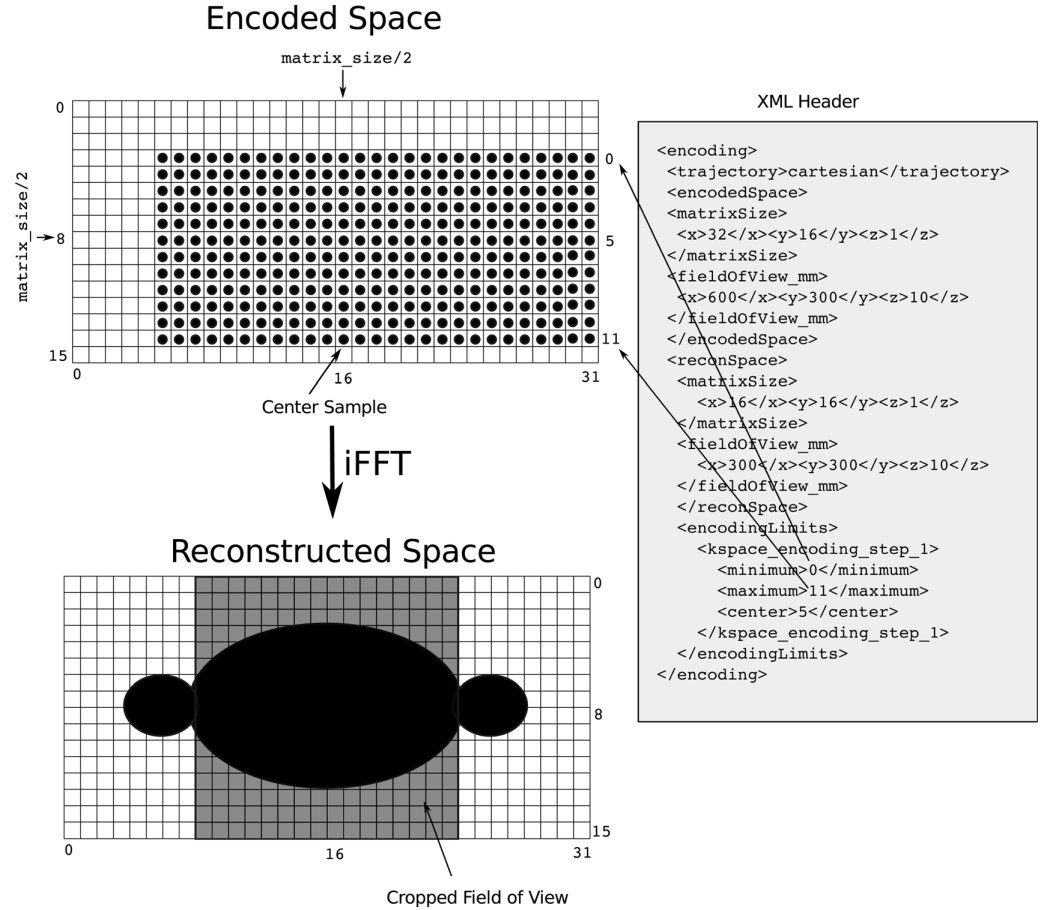
\includegraphics[width=0.7\linewidth]{chapters/chapter-2/figs/ismrmrd-encodedSpace}
	}{\doiSource{10.1002/mrm.26089}}
	\caption{}
	\label{fig:ismrmrd-encodedspace}
\end{figure}




\begin{table}[b!]
	\begin{latin}\footnotesize
	\begin{tabularx}{\linewidth}{lXXXX}
	\hline
	ISMRMRD & Bruker & GE & Philips & Siemens \\ \hline
	kspace\_encode\_step\_1 & encode step 1 &‌ Frame&‌ e1 & Line\\
	kspace\_encode\_step\_2 & encode step 2 &‌ – &‌ e2 &‌ Partition\\
	Average & – & – &  Measurement & Acquisition\\
	Slice & Slice‌&  Slice &  Location & Slice \\
	Contrast &‌ Echo &‌ Echo & Echo & Echo\\
	Phase &‌ ‌– &‌ – &‌ Cardiac phase & Phase\\
	Repetition & Repetition &‌ Repetition&‌ Dynamic scan& Repetition\\
	Set & – & – &‌Row& Set\\
	Segment & – & – & – & Segment\\ \hline
	\end{tabularx}
	\end{latin}
\caption{}
\end{table}

